\documentclass[11pt, a4paper]{article}

% --- 页面设置 ---
\usepackage[a4paper, top=2.5cm, bottom=2.5cm, left=2cm, right=2cm]{geometry}

% --- [核心修正] 中文支持方案 ---
% 使用 ctex 宏包替代 babel。这是处理中文最标准、最稳妥的方式。
% 注意：请务必继续使用 XeLaTeX 编译器。
\usepackage[heading=true]{ctex}

% 列表样式优化
\usepackage{enumitem}
\setlist[itemize]{label=-}

% --- 其他必要的宏包 ---
\usepackage{amsmath}    % 数学公式
\usepackage{booktabs}   % 专业表格 (三线表)
\usepackage{listings}   % 代码展示
\usepackage{xcolor}     % 颜色支持
\usepackage{graphicx}   % 图片支持
\usepackage{float}      % 浮动体控制 (用于 [H] 强行固定图片位置)

% --- 代码高亮设置 (MATLAB 风格) ---
\definecolor{codegreen}{rgb}{0,0.6,0}
\definecolor{codegray}{rgb}{0.5,0.5,0.5}
\definecolor{codepurple}{rgb}{0.58,0,0.82}
\definecolor{backcolour}{rgb}{0.95,0.95,0.92}

\lstset{
	language=Matlab,
	backgroundcolor=\color{backcolour},   
	commentstyle=\color{codegreen},
	keywordstyle=\color{blue},
	numberstyle=\tiny\color{codegray},
	stringstyle=\color{codepurple},
	basicstyle=\ttfamily\footnotesize,
	breakatwhitespace=false,         
	breaklines=true,                 
	captionpos=b,                    
	keepspaces=true,                 
	numbers=left,                    
	numbersep=5pt,                  
	showspaces=false,                
	showstringspaces=false,
	showtabs=false,                  
	tabsize=2,
	frame=single,
	% 解决代码中包含中文注释可能显示乱码或报错的问题
	escapeinside=``
}

% --- 文档信息 ---
\title{\textbf{实验三 \quad 非线性支持向量机实验报告}}
\author{姓名：\underline{\makebox[3cm]{林鑫}} \quad 学号：\underline{\makebox[3cm]{1043220122}}}
\date{\today}

\begin{document}
	
	\maketitle
	
	\section{实验目的}
	\begin{itemize}
		\item 理解支持向量机（SVM）的基本原理，特别是针对非线性可分数据的核函数方法。
		\item 掌握将SVM对偶问题转化为二次规划标准型的方法，并利用MATLAB优化工具箱（\texttt{quadprog}函数）求解。
	\end{itemize}
	
	\section{实验内容}
	现有5个一维数据样本：
	\begin{itemize}
		\item \textbf{第一类 (Class 1, $y=1$):} $x_1=1, x_2=2, x_5=6$
		\item \textbf{第二类 (Class 2, $y=-1$):} $x_3=4, x_4=5$
	\end{itemize}
	
	要求选择多项式核函数（Polynomial kernel of degree 2），公式为 $K(x,y) = (xy + 1)^2$，惩罚参数 $C=100$。
	
	\textbf{实验任务：}
	\begin{enumerate}
		\item 求解支持向量机的拉格朗日乘子 $\alpha_i \ (i=1,\dots,5)$。
		\item 求解偏置项 $b$。
		\item 利用求得的非线性模型，对测试数据 $X_6=3$ 和 $X_7=8$ 进行分类预测。
		\item 对分类结果及决策函数进行可视化展示。
	\end{enumerate}
	
	\begin{table}[htbp]
		\centering
		\caption{实验数据表}
		\begin{tabular}{cccc}
			\toprule
			样本编号 & 特征值 ($X$) & 标签 ($Y$) & 类别 \\
			\midrule
			1 & 1 & 1 & Class 1 \\
			2 & 2 & 1 & Class 1 \\
			3 & 4 & -1 & Class 2 \\
			4 & 5 & -1 & Class 2 \\
			5 & 6 & 1 & Class 1 \\
			\bottomrule
		\end{tabular}
	\end{table}
	
	\section{问题解答}
	本题是一个带约束条件的凸二次规划问题（软间隔SVM的对偶形式）。决策变量是拉格朗日乘子 $\alpha = [\alpha_1, \alpha_2, \alpha_3, \alpha_4, \alpha_5]^T$。
	
	\subsection{目标函数}
	对偶问题的最小化形式为：
	\begin{equation}
		\min_{\alpha} \left( \frac{1}{2} \sum_{i=1}^{5}\sum_{j=1}^{5} \alpha_i \alpha_j y_i y_j K(x_i, x_j) - \sum_{i=1}^{5} \alpha_i \right)
	\end{equation}
	其中核矩阵元素 $K(x_i, x_j) = (x_i x_j + 1)^2$。
	
	\subsection{约束条件}
	\begin{itemize}
		\item \textbf{等式约束：} $\sum_{i=1}^{5} \alpha_i y_i = 0$
		\item \textbf{不等式约束：} $0 \le \alpha_i \le C$ （其中 $C=100$）
	\end{itemize}
	
	\subsection{MATLAB 参数映射}
	将二次规划写成 MATLAB \texttt{quadprog} 的标准形式：
	\begin{itemize}
		\item \textbf{H 矩阵：} $H_{ij} = y_i y_j K(x_i, x_j)$
		\item \textbf{f 向量：} $f = [-1, -1, -1, -1, -1]^T$
		\item \textbf{等式约束：} $A_{eq} = Y^T, \ b_{eq} = 0$
		\item \textbf{边界约束：} $lb = 0, \ ub = 100$
	\end{itemize}
	
	\section{MATLAB 程序}
	\begin{lstlisting}[caption={非线性SVM求解及可视化脚本}]
		clear; clc;
		% --- 1. 核心算法求解 ---
		X = [1; 2; 4; 5; 6];      
		Y = [1; 1; -1; -1; 1];    
		C = 100;                  
		n = length(Y);            
		
		% 计算核矩阵及H矩阵
		K = zeros(n, n);
		for i = 1:n
		for j = 1:n
		K(i,j) = (X(i) * X(j) + 1)^2;
		end
		end
		H = (Y * Y') .* K; 
		
		% 二次规划参数
		f = -ones(n, 1);          
		Aeq = Y'; beq = 0;
		lb = zeros(n, 1); ub = C * ones(n, 1);
		
		% 求解 alpha
		options = optimoptions('quadprog', 'Display', 'off');
		alpha = quadprog(H, f, [], [], Aeq, beq, lb, ub, [], options);
		
		% 计算偏置 b
		epsilon = 1e-5;
		sv_indices = find(alpha > epsilon & alpha < (C - epsilon));
		if isempty(sv_indices), sv_indices = find(alpha > epsilon); end
		k = sv_indices(1);
		sum_wx = 0;
		for i = 1:n
		sum_wx = sum_wx + alpha(i) * Y(i) * K(i, k);
		end
		b = Y(k) - sum_wx;
		
		% 输出参数
		disp('求解得到的 alpha:'); disp(alpha);
		disp(['求解得到的 b: ', num2str(b)]);
		
		% --- 2. 可视化部分 ---
		figure('Name', 'SVM可视化', 'Color', 'w'); hold on; box on; grid on;
		x_plot = 0:0.05:9; 
		f_plot = zeros(size(x_plot));
		for j = 1:length(x_plot)
		x_val = x_plot(j);
		wx = 0;
		for i = 1:n
		k_val = (X(i) * x_val + 1)^2; 
		wx = wx + alpha(i) * Y(i) * k_val;
		end
		f_plot(j) = wx + b;
		end
		% 绘制决策函数曲线
		plot(x_plot, f_plot, 'k-', 'LineWidth', 2);
		yline(0, 'k--', 'LineWidth', 1.5); % 决策边界
		
		% 绘制样本点和支持向量
		idx1 = find(Y == 1); idx2 = find(Y == -1);
		plot(X(idx1), zeros(size(idx1)), 'bo', 'MarkerFaceColor', 'b');
		plot(X(idx2), zeros(size(idx2)), 'rs', 'MarkerFaceColor', 'r');
		plot(X(sv_indices), zeros(size(sv_indices)), 'ko', 'MarkerSize', 12, 'LineWidth', 1.5);
		
		% 绘制测试数据
		X_test = [3; 8];
		test_vals = zeros(size(X_test));
		for j = 1:length(X_test)
		x_target = X_test(j);
		val = 0;
		for i = 1:n
		k_val = (X(i) * x_target + 1)^2; 
		val = val + alpha(i) * Y(i) * k_val;
		end
		test_vals(j) = val + b;
		end
		plot(X_test, test_vals, 'mh', 'MarkerSize', 12, 'MarkerFaceColor', 'm');
		
		xlabel('特征值 X'); ylabel('决策函数值 f(x)');
		title(['SVM 多项式核(d=2) 分类结果 (C=' num2str(C) ')']);
	\end{lstlisting}
	
	\section{计算结果}
	
	\subsection{求解得到的 Alpha 值}
	\begin{table}[htbp]
		\centering
		\caption{拉格朗日乘子 $\alpha$ 求解结果}
		\begin{tabular}{ccl}
			\toprule
			$i$ & Alpha 值 ($\alpha_i$) & 说明 \\
			\midrule
			1 & 0.0000 & 非支持向量 \\
			2 & 2.5000 & \textbf{支持向量} \\
			3 & 0.0000 & 非支持向量 \\
			4 & 7.3333 & \textbf{支持向量} \\
			5 & 4.8333 & \textbf{支持向量} \\
			\bottomrule
		\end{tabular}
	\end{table}
	
	\subsection{求解得到的偏置项 b}
	\begin{table}[htbp]
		\centering
		\caption{偏置项 $b$ 求解结果}
		\begin{tabular}{cc}
			\toprule
			参数 & 计算值 \\
			\midrule
			偏置 $b$ & 9.0000 \\
			\bottomrule
		\end{tabular}
	\end{table}
	
	\subsection{测试数据分类预测结果}
	\begin{table}[htbp]
		\centering
		\caption{测试数据分类预测}
		\begin{tabular}{ccc}
			\toprule
			测试样本 $X$ & 决策函数值 $f(x)$ & 预测类别 \\
			\midrule
			3 & -1.000000 & Class 2 \\
			8 & 9.000000 & Class 1 \\
			\bottomrule
		\end{tabular}
	\end{table}
	
	\subsection{可视化结果}
	\begin{figure}[H]
		\centering
		% [重要] 请确保图片文件名与此处一致，并放在同一目录下
		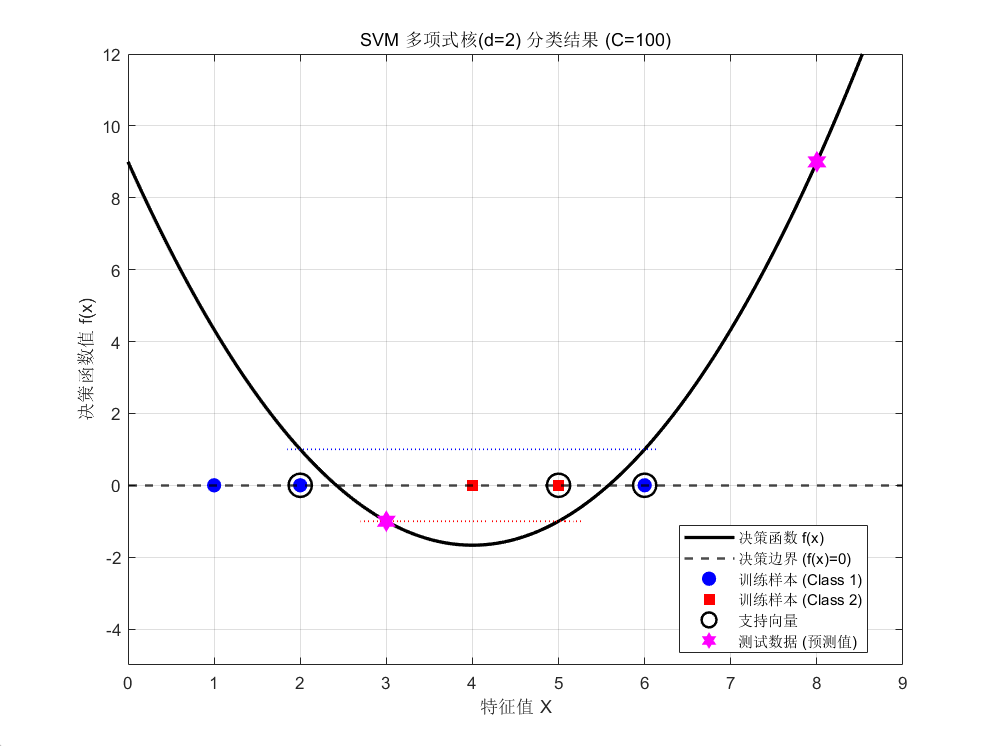
\includegraphics[width=0.8\textwidth]{svm_vis_result.png}
		\caption{SVM 非线性分类决策函数曲线及样本分布。图中黑色曲线为决策函数 $f(x)$，虚线为决策边界 $f(x)=0$。蓝色圆点和红色方块分别为两类训练样本，黑色圆圈圈出的点为支持向量。粉色六角星为测试数据点。}
		\label{fig:svm_vis}
	\end{figure}
	
	\section{结果分析}
	\begin{enumerate}
		\item \textbf{支持向量分析：} 从结果 $\alpha$ 可以看出，$\alpha_2=2.5$, $\alpha_4=7.3333$, $\alpha_5=4.8333$ 明显大于0，说明对应的样本 $x_2=2$, $x_4=5$, $x_5=6$ 是该模型的支持向量，它们决定了决策边界的位置。
		
		\item \textbf{分类结果验证：}
		\begin{itemize}
			\item 对于 \textbf{$X=3$}：其位置介于 $x_2=2$ (Class 1) 和 $x_3=4$ (Class 2) 之间。如图\ref{fig:svm_vis}所示，测试点（粉色六角星）位于决策边界下方（$f(x)<0$），因此被判定为 Class 2。
			\item 对于 \textbf{$X=8$}：其位置在 $x_5=6$ (Class 1) 的右侧。如图\ref{fig:svm_vis}所示，测试点位于决策函数曲线上升区（$f(x)>0$），因此被判定为 Class 1。
		\end{itemize}
		
		\item \textbf{参数检验：} 
		验证 KKT 条件中的等式约束 $\sum_{i=1}^{5} \alpha_i y_i = 0$：
		\[
		2.5(1) + 7.3333(-1) + 4.8333(1) = 7.3333 - 7.3333 \approx 0
		\]
		计算结果满足约束条件，说明求解有效。
	\end{enumerate}
	
\end{document}